%!TEX program = xelatex
\documentclass[aspectratio=169]{ctexbeamer}
% \usepackage{physics}  
                        %%% 宽高比说明 %%%%
%% ctexbeamer宏包支持各种宽高比,但本模板只适配了4:3(默认)和16:9的宽高比背景。
%% 添加选项aspectratio=169或aspectratio=43可以更改宽高比,默认是4:3
\usepackage[bluetheme]{ustcbeamer}
\input{ustctheme.tex}
                        %%% ustcbeamer说明 %%%%
%% 宏包使用了TikZ代码形式的背景文件(在子文件夹theme中),默认选项"bluetheme",是科大校徽的蓝色;此外ustcbeamer还内置了红色和黑色主题"redtheme","blacktheme"。

                        %%% 自定义你的主题颜色 %%%
%% 一旦使用了下述命令就会覆盖ustcbeamer的内置颜色选项,你可以设置自己喜欢的RGB色值:
% \definecolor{themecolor}{RGB}{0,150,0} % 这是绿色主题
% \definecolor{themecolor}{RGB}{0,150,150} % 青色主题,也蛮好看的

%% 注意小写rgb和大写RGB表示的色值相差255倍,即RGB{255,255,255}=rgb{1,1,1};
% \definecolor{themecolor}{rgb}{0,0.5,0.3} % 深绿色主题

%% 建议自定义的主题颜色选择偏深色
%%%%%%%%%%%%%%%%%%%%%%%%%%%%%%%%%%%%%%%%%%%%%%%%%%%%%%%%%%%%%%%%%%%%%%


\title[基于生成式先验的肖像视频编辑系统的设计与实现]{
    基于生成式先验的肖像视频编辑系统的设计与实现
}
\author[汪兆辰]{报告人:汪兆辰\\指导教师:张举勇教授}
\institute[USTC]{
数学科学学院·计算与应用数学系
}
\date{\today}
\begin{document}
%\section<⟨mode specification⟩>[⟨short section name⟩]{⟨section name⟩}
%小于等于六个标题为恰当的标题

%--------------------
%标题页
%--------------------
\maketitleframe
%--------------------
%目录页
%--------------------
%beamer 101
\begin{frame}%
	\frametitle{目录}%
	\tableofcontents[hideallsubsections]%仅显示节
	%\tableofcontents%显示所节和子节
\end{frame}%
%--------------------
%节目录页
%--------------------
\AtBeginSection[]{
\setbeamertemplate{footline}[footlineoff]%取消页脚
  \begin{frame}%
    \frametitle{目录}
	%\tableofcontents[currentsection,subsectionstyle=show/hide/hide]%高亮当前节,不显示子节
    \tableofcontents[currentsection,subsectionstyle=show/show/hide]%show,shaded,hide
  \end{frame}
\setbeamertemplate{footline}[footlineon]%添加页脚
}
%--------------------
%子节目录页
%--------------------
\AtBeginSubsection[]{
\setbeamertemplate{footline}[footlineoff]%取消页脚
  \begin{frame}%
    \frametitle{目录}
	%\tableofcontents[currentsection,subsectionstyle=show/hide/hide]%高亮当前节,不显示子节
    \tableofcontents[currentsection,subsectionstyle=show/shaded/hide]%show,shaded,hide
  \end{frame}
\setbeamertemplate{footline}[footlineon]%添加页脚
}

\section{研究背景与意义}
\begin{frame}
  \frametitle{研究背景}
  \begin{itemize}
    \item \textbf{行业需求:}
    \begin{itemize}
      \item 中国网络视听用户规模已达 10.91 亿,其中短视频用户规模突破 10.40 亿,日均使用时长高达 156 分钟;
      \item 我国网络直播用户规模达 8.33 亿,同比增长1737 万;
      \item 2024 年全国网上零售额达 15.23 万亿元,同比增长 7.2\%,其中近一半的消费行为直接由短视频或直播内容触发。
    \end{itemize}
    \item \textbf{技术挑战:}
    \begin{itemize}
      \item 传统的基于2D先验的编辑方法无法满足视频多样化编辑的需求;
      \item 现有先进编辑技术的应用门槛较高,普通用户难以直接使用;
      \item 研究者难以获得用户的实际需求,造成技术演进与市场需求的脱节。
    \end{itemize}
  \end{itemize}
\end{frame} 

\begin{frame}
  \frametitle{研究意义}
  \begin{itemize}
    \item 我们基于PortraitGen算法,构建了一套完整的智能视频编辑系统,设计了直观的用户界面与用户工作流,使用户
    无需关注算法细节,只需给出算法输入便可实现多种编辑功能。
    \item 另外我们搭建了管理员系统,使研究者可以监控用户反馈和操作日志,从而了解用户需求。
    \item 我们在构建系统时保持了可扩展性,为搭载多种算法提供可能。
  \end{itemize}

\end{frame}

\section{相关技术与工作}

\begin{frame}
  \frametitle{PortritGen技术创新}
  我们使用的PortraitGen算法将肖像表示提升至3D以保持生成视频帧间的一致性,其主要技术创新在于:
  \begin{itemize}
    \item 通过3DGS来表示肖像,提高模型表示能力;
    \item 使用可学习的特征代替球谐系数,实现更精细的艺术细节;
    \item 利用表情一致性保持策略,增强面对复杂问题的稳定性。
  \end{itemize}
  \begin{figure}
    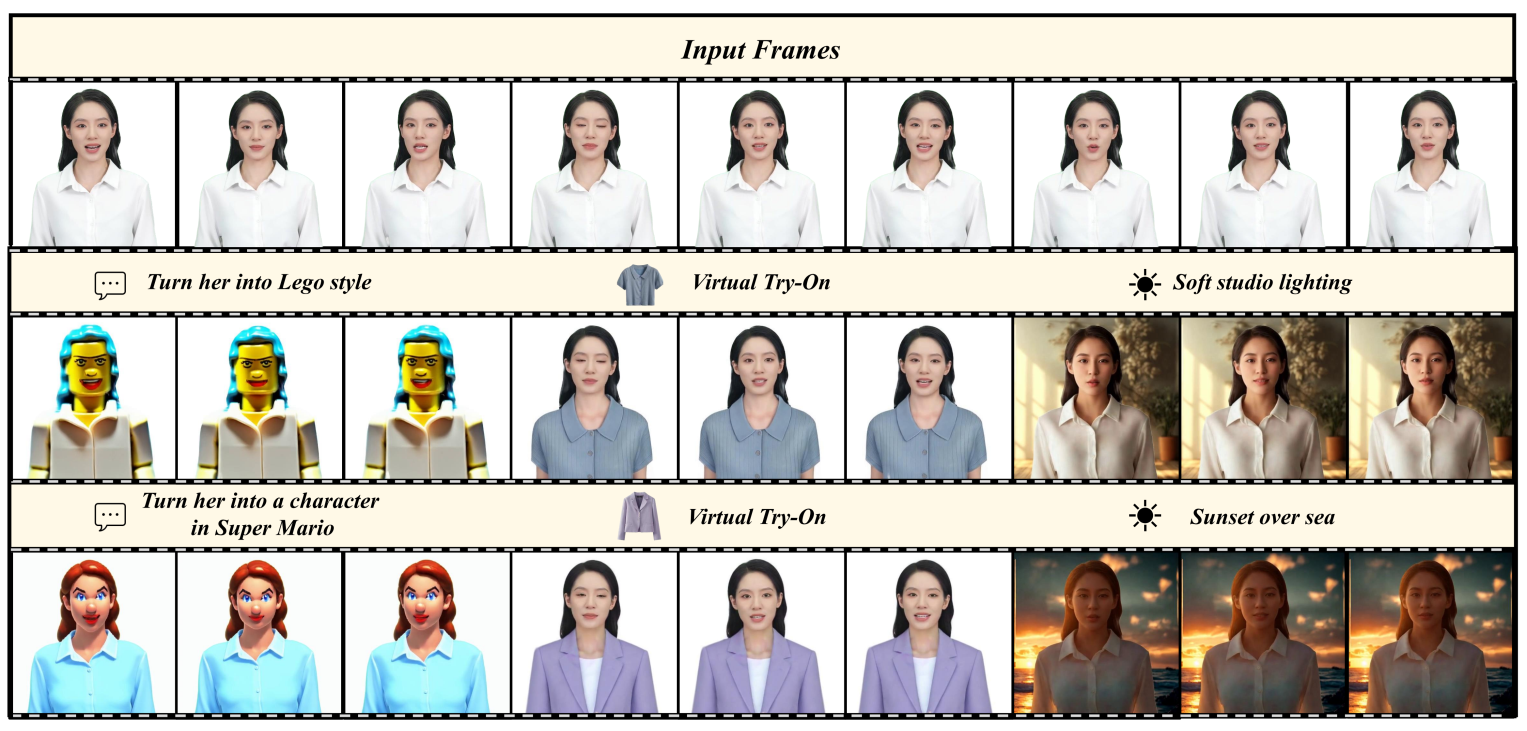
\includegraphics[width=0.5\textwidth]{source/portraitgen.png}
  \end{figure}
\end{frame}

\begin{frame}
  \frametitle{系统开发技术}
  我们采用前后端分离的分层微服务架构搭建系统:
  \begin{columns}
    \begin{column}{0.4\textwidth}
      \begin{itemize}
        \item 使用基于React的Next.js作为前端开发框架,并选择Typescript以引入类型检查与对象特性;
        \item 后端API使用Flask框架以适配算法并提供可扩展的微服务;
        \item 数据层采用MySQL存储数据,Redis实现任务队列管理。
      \end{itemize}
    \end{column}
    \begin{column}{0.6\textwidth}
      \begin{figure}
        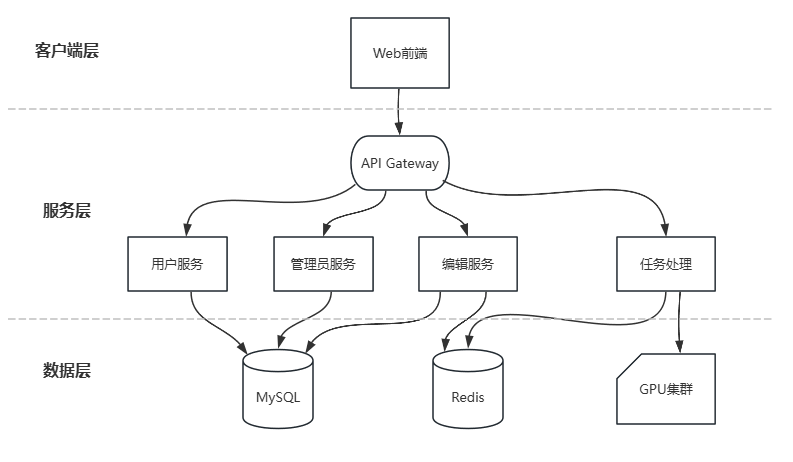
\includegraphics[width=0.9\textwidth]{source/system_structure.png}
      \end{figure}
    \end{column}
  \end{columns}
\end{frame}

\section{系统设计与实现}
\subsection{需求分析}
\begin{frame}
  \frametitle{需求分析}
  
\end{frame}


\section{总结展望}

\begin{frame}
  \frametitle{总结展望}
  \begin{columns}
    \begin{column}{0.50\textwidth}
      \begin{figure}
        \includegraphics[width=0.8\textwidth]{figures/ustc_logo.pdf}
        \caption{标题}
      \end{figure}
    \end{column}
    \begin{column}{0.50\textwidth}
      \begin{block}{结论}
        \begin{itemize}
          \item 结论 1
          \item 结论 2
          \item 结论 3
        \end{itemize}
      \end{block}
    \end{column}
  \end{columns}
\end{frame}

\begin{frame}
  \frametitle{致谢}
  \centerline{\Large 谢谢!}
\end{frame}

\end{document}
